% !TeX spellcheck = en_US
\documentclass{article}
\usepackage{graphicx}
\usepackage{fancybox}
\usepackage{tikz}
\usepackage{algorithm}
\usepackage{amsmath}
\usepackage{algorithmicx}
\usepackage{hyperref}
\usepackage{algpseudocode}
\usepackage{graphicx}
\usepackage{caption}

\captionsetup{labelfont={color=black,bf}}

\makeatletter
\def\BState{\State\hskip-\ALG@thistlm}
\makeatother

\algdef{SE}[DOWHILE]{Do}{doWhile}{\algorithmicdo}[1]{\algorithmicwhile\ #1}%

\title{Homework 06: Weighted Graphs}
\date{\today}
\author{Roberto Corti}

\begin{document}
	
	\maketitle
	
	\section*{Exercise 1}
	\textbf{Implement the array-based version of the Dijkstra’s algorithm.}\\
	
	\noindent The implementation of the array-based version of the Dijkstra’s algorithm can be found in the code \texttt{src/dijkstra.c} in the function \texttt{dijkstra}. 
	
	
	\section*{Exercise 2}
	\textbf{Implement the binary heap-based version of the Dijkstra’s algorithm by using the library \texttt{binheap} that was developed during Lesson 6, Lesson 7 and Lesson 8.}\\
	
	\noindent The implementation of the heap-based version of the Dijkstra’s algorithm can be found in the code \texttt{src/dijkstra.c} in the function \texttt{dijkstra\_heap}. In order to build a priority queue based on a heap I used the implementation of the binary heap done in the Homework 03, which provides an array-based implementation of binary heaps that avoids to swap the elements in the array.
	
	\section*{Exercise 3}
	\textbf{Test the implementations on a set of instances of the problem and compare their execution times.}\\ 
	
	\noindent Once provided the correctness of the previous two implementations I proceeded to test the performance of these two versions of the Dijkstra's Algorithm. The following plot in Figure 1 reports the result.
	\newpage
	\begin{figure}[th]
			\centering
			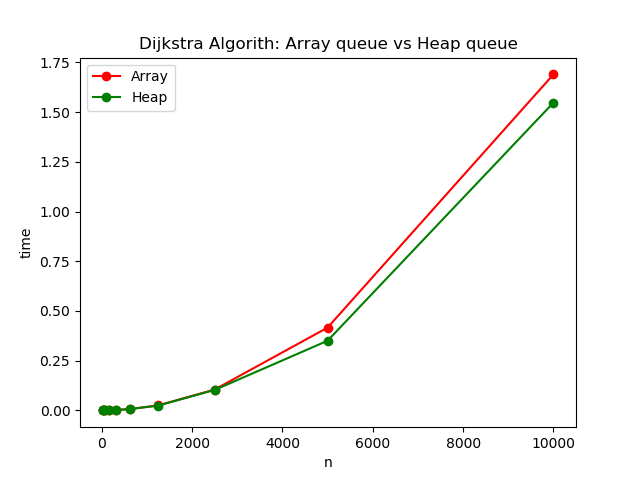
\includegraphics[width=.7\textwidth]{../plot/plot.png}
			\label{plot}
			\caption{Time performance of the two implementations of the Dijkstra's Algorithm}
	\end{figure}
	\noindent The plot shows that the heap version performs better than the array version, especially for larger sizes. This is expected, since the asymptotic complexity of the first version is $\Theta(|V|^2 + |E|)$, while the second is $O ( (|V| + |E| ) \cdot \log{(|V|)} )$  \footnote{$|V|$ and $|E|$ are respectively the number of the vertex and the edges inside a graph.}.

\end{document}

